% Build from the repository root: ./scripts/build_delivery.sh
% Report prose is maintained here; author identity comes from author.txt.
\documentclass[10pt,a4paper]{article}
\usepackage[T1]{fontenc}
\usepackage[utf8]{inputenc}
\usepackage{lmodern}
\usepackage[a4paper,margin=15mm,footskip=8mm]{geometry}
\usepackage{graphicx,xcolor,amsmath,microtype,fancyhdr}
\usepackage{titlesec}
\usepackage[hidelinks]{hyperref}
\hypersetup{pdftitle={Foundation: economic dependency and widespread control}}
\DeclareUnicodeCharacter{2192}{\ensuremath{\rightarrow}}
\DeclareUnicodeCharacter{2194}{\ensuremath{\leftrightarrow}}
\DeclareUnicodeCharacter{2265}{\ensuremath{\geq}}
\DeclareUnicodeCharacter{00D7}{\ensuremath{\times}}
\DeclareUnicodeCharacter{2212}{\ensuremath{-}}
\DeclareUnicodeCharacter{00B1}{\ensuremath{\pm}}
\definecolor{navy}{HTML}{142B42}
\definecolor{teal}{HTML}{087F8C}
\definecolor{pale}{HTML}{EDF5F6}
\color{navy}
\setlength{\parindent}{0pt}
\setlength{\parskip}{4pt}
\titleformat{\section}{\large\bfseries\color{teal}}{}{0pt}{}
\titlespacing*{\section}{0pt}{8pt}{4pt}
\pagestyle{fancy}
\fancyhf{}
\fancyfoot[R]{\footnotesize\thepage\ / 2}
\renewcommand{\headrulewidth}{0pt}
\renewcommand{\footrulewidth}{0pt}
\graphicspath{{../results/tipping_point_investigation/figures/}}
\newcommand{\reporttitle}[1]{{\Large\bfseries\color{teal}#1\par}\vspace{3pt}}
\newcommand{\figurecaption}[1]{{\footnotesize #1\par}}
\begin{document}


\reporttitle{Foundation: influence through economic dependency}
{\footnotesize\input{author.txt} • Collective Intelligence • Assignment 1 • Autumn 2026\par}

\section*{Motivation and research question}

Isaac Asimov’s \emph{Foundation} inspires a fictional model of non-military expansion: missionaries maintain advanced devices and religious institutions, while traders create dependence on imported technology. How do trader population and trade attractiveness influence widespread Foundation control? The hypothesis is that more frequent, attractive trade raises dependency and trust enough to establish broad leverage under favorable missionary conditions. This is an original fictional abstraction, not a predictive representation of real societies.


\section*{Agents and interactions}

The 64 × 64 toroidal world contains 31 stationary planets: Terminus, four kingdoms of five planets each (one capital per kingdom), and ten independent markets. Two traveling breeds interact with planets: missionaries and traders. Stochastic destination choice favors accessible, useful nearby worlds but includes exploration. Accepted missions increase religion with saturation; established temples support religion and device maintenance. Religion improves trade admission without making conversion mandatory. Successful sales raise technological dependency, infrastructure health and trust, create or reinforce trade routes, and generate revenue. Deaths and paid recruitment constrain staffing.


\section*{ODD overview and dynamic environment}

\textbf{Purpose and state:} study emergent, reversible leverage; planets hold religion, dependency, demand, health, wealth, hostility and policy, travelers hold skill and destination, and routes hold strength and age. \textbf{Initialization:} a random separated galaxy and heterogeneous bounded planet states; open governments, no routes or controlled worlds; no external input data. \textbf{Scheduling:} environment → missions → trade → route wear → government/recruitment every ten ticks → local political effects → control → clock. \textbf{Design concepts:} saturation, stochastic admission, economic feedback, policy hysteresis and emergent networks. Demand regenerates, technology degrades, local substitutes reduce dependence and unused routes disappear. Capitals can impose restrictions or embargoes; dependency and falling wealth can induce concessions. Kingdom names do not script victory.


\section*{Control, parameters and interface}

Planet leverage is clamp01(0.30 religion + 0.35 dependency + 0.25 trust + 0.15(1 − hostility)). Leverage ≥0.58 for five consecutive ticks establishes effective control; a lower tick removes it. A kingdom requires its controlled capital and ≥60\% of its population on controlled worlds. Control is influence, not sovereignty. Control fraction counts the 30 external planets only.


Key controls are missionary effectiveness, missionary staffing, trader staffing, trade attractiveness, royal intolerance, technology decay, religion-assisted trade admission and local substitution. The confirmatory settings are effectiveness 0.50, missionaries 12, intolerance 0, decay 0.015, religion-trade weight 0.80 and independence effort 0.15; traders and attractiveness vary on page 2. The ninth slider sets duration: interactive default 0 means unlimited, while experiments capture a finite limit at setup.


The self-contained NetLogo 6.4 model provides setup, go-once and go; four planet views; twelve monitors; control, influence and trade time series; and a religion histogram. The Info tab supplies the full ODD and equations. No warfare, empirical calibration or individual worshippers are modeled; space and credits are abstract.


{\footnotesize \textbf{References and authorship:} Asimov, I. (1951), \emph{Foundation} (literary inspiration); Wilensky, U. (1999), \emph{NetLogo}, Northwestern University; Takács, T. (2026), Assignment 1. AI assistance was used for code, documentation and delivery.\par}

\vfill
\noindent
\colorbox{pale}{\parbox[c][7mm][c]{0.30\linewidth}{\centering\footnotesize\color{teal}Missions → religion}}\hfill
\colorbox{pale}{\parbox[c][7mm][c]{0.30\linewidth}{\centering\footnotesize\color{teal}Trade → dependency}}\hfill
\colorbox{pale}{\parbox[c][7mm][c]{0.30\linewidth}{\centering\footnotesize\color{teal}Leverage ↔ resistance}}
\newpage
\reporttitle{Experiment, measured results and interpretation}
\fontsize{9}{11}\selectfont


BehaviorSpace varies \textbf{initial-traders} \{8, 12, 16, 20, 24\} × \textbf{trade-attractiveness} \{0.60, 0.80, 1.00\}: 15 cells, 20 repetitions each, 300 runs at 1,000 ticks. XML: \textbf{tipping\_confirmatory.xml}; seeds 500000 + run number. Fixed settings are on page 1. The earlier 980-run missionary × intolerance sweep found no widespread control; separate duration, mechanism-screening and boundary-search experiments selected these ranges. Exploratory and confirmatory observations are not pooled.


Primary outcomes are final control fraction and controlled kingdoms (0–4); per-cell means and 95\% Student t intervals use df=19. Widespread control means final fraction ≥0.50 (≥15/30 worlds); its probability uses 95\% Wilson binomial intervals.


\begin{center}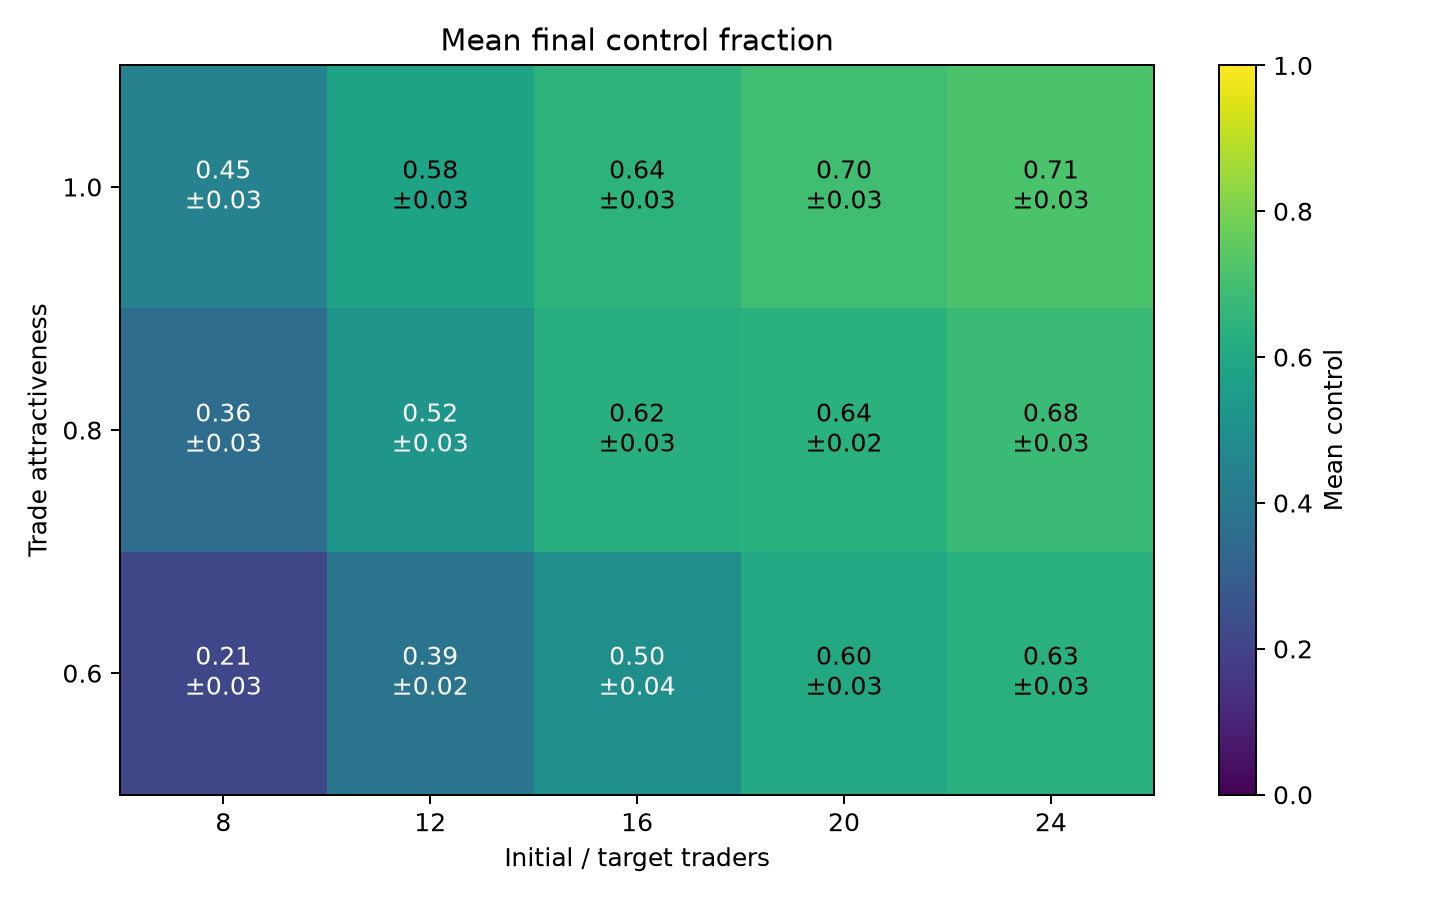
\includegraphics[width=0.88\linewidth,height=76mm,keepaspectratio]{control_heatmap.png}\end{center}

\figurecaption{Figure 1. Mean final control fraction; each cell shows mean ±95\% t CI half-width. Color spans 0–1. The 50\% criterion is an operational definition, not a universal constant.}

\begin{center}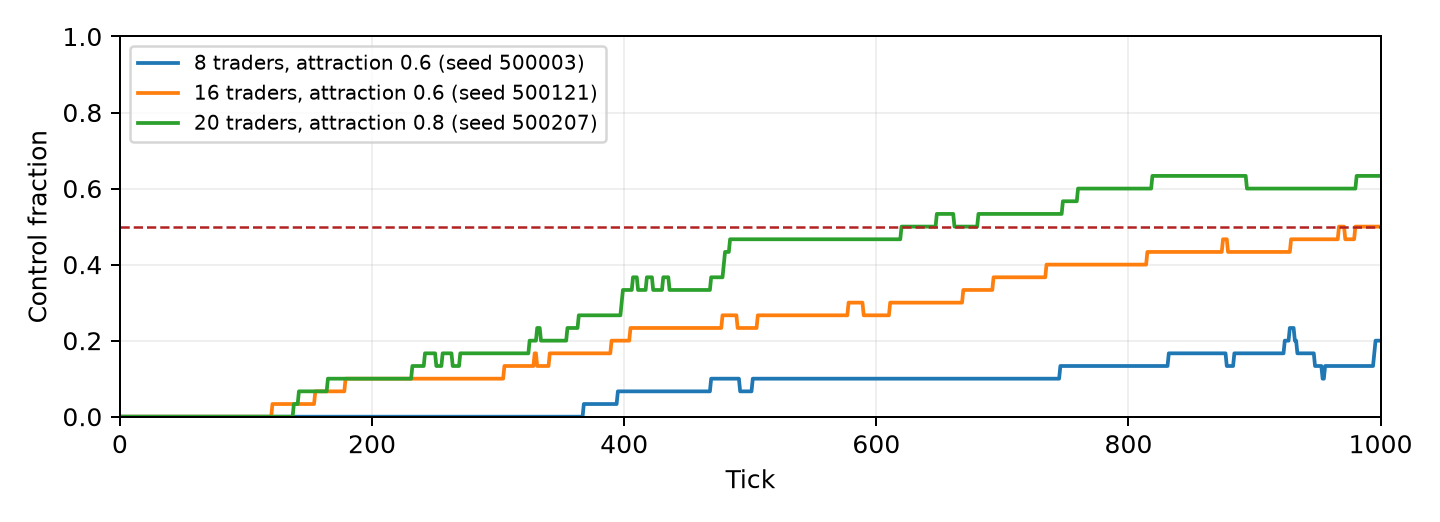
\includegraphics[width=\linewidth,height=46mm,keepaspectratio]{representative_control_timeseries.png}\end{center}

\figurecaption{Figure 2. Genuine below/near/above-boundary confirmatory replays. Dashed line: 50\% criterion. Seeds 500003, 500121, 500207; final states 0.200, 0.500, 0.633. The last case uses attractiveness 0.80; the other two use 0.60.}

At attractiveness \textbf{0.60}, 12 traders yield \textbf{0/20} widespread runs and mean 0.387 [0.364, 0.409]; 16 yield \textbf{10/20} and 0.497 [0.460, 0.533]; 20 yield \textbf{20/20} and 0.605 [0.577, 0.633]. Corresponding Wilson intervals are [0.000, 0.161], [0.299, 0.701], [0.839, 1.000]. At 0.80, 12 traders yield 16/20, moving the boundary toward fewer traders. More trade increases dependency and trust, strengthening leverage. Kingdom-count means and intervals are retained in the processed CSV.


The crossing probability changes rapidly between 12 and 20 traders at 0.60, while continuous control grows more smoothly: an \textbf{operational stochastic threshold}, not proof of a mathematical phase transition. The near-boundary replay first crosses at tick 967 and is widespread in only 26/1,001 states; terminal crossing does not establish persistence. The above-boundary replay is widespread throughout the final 100 ticks.


\textbf{Takeaway:} favorable missionary access enables expansion, but sufficiently strong economic ties drive widespread control in this model. \textbf{Limits:} fictional coefficients, favorable fixed politics, finite horizon, coarse four-trader spacing, twenty runs and selection after exploratory search restrict generality. Future work: fresh 14/18-trader validation cells and persistence measurements across all runs.


\end{document}
